\documentclass[12pt]{article}
\usepackage{array}
\usepackage{amsmath}
\usepackage{mathtools}
\usepackage{gensymb}
\usepackage{graphicx}
\usepackage{float}
\usepackage{caption}
\usepackage{setspace}


\allowdisplaybreaks

\begin{document}

    \title{Equipotentials and the Electric Field}
    \author{Ryan Coyne, Ben Eid, Erin Snook}
    \maketitle

    \section{Abstract}
        In this lab, we inserted electrodes into conducting paper with metallic ink arranged to create particular charge configurations. The conducting paper was on top of white grid paper, and they were pinned to foam board. The electrodes created an electric field in the conducting paper, and the electric potential could be measured by touching the conducting paper with the volt meter. Lightly pressing the electrode of the voltmeter into the conducting paper left indentations in the grid paper. 
        
        After making indentations at 1-volt intervals so that the equipotentials were clear, the papers were removed from the foam. Lines marking the equipotentials were drawn between the indentations on the grid paper, and then electric field lines were drawn to be orthogonal to the equipotentials. The distance between two equipotentials was measured on each grid paper in particular locations. The strength of the electric field was estimated at those locations using the equation
        \begin{equation*}
            E = \frac{\Delta V}{\Delta s}
        \end{equation*}
        where \(E\) is the electric field strength, \(\Delta V\) is the difference between the electric potential, and \(\Delta s\) is the distance between the electric potentials.

        Overall the results matched my intuition, the only exception was in Figure 2, where the electric field seems to deflect in a way that I wouldn't expect below the dielectric at the 2 V equipotential.
    \section{Data}
        \begin{figure}[H]
            \centering
            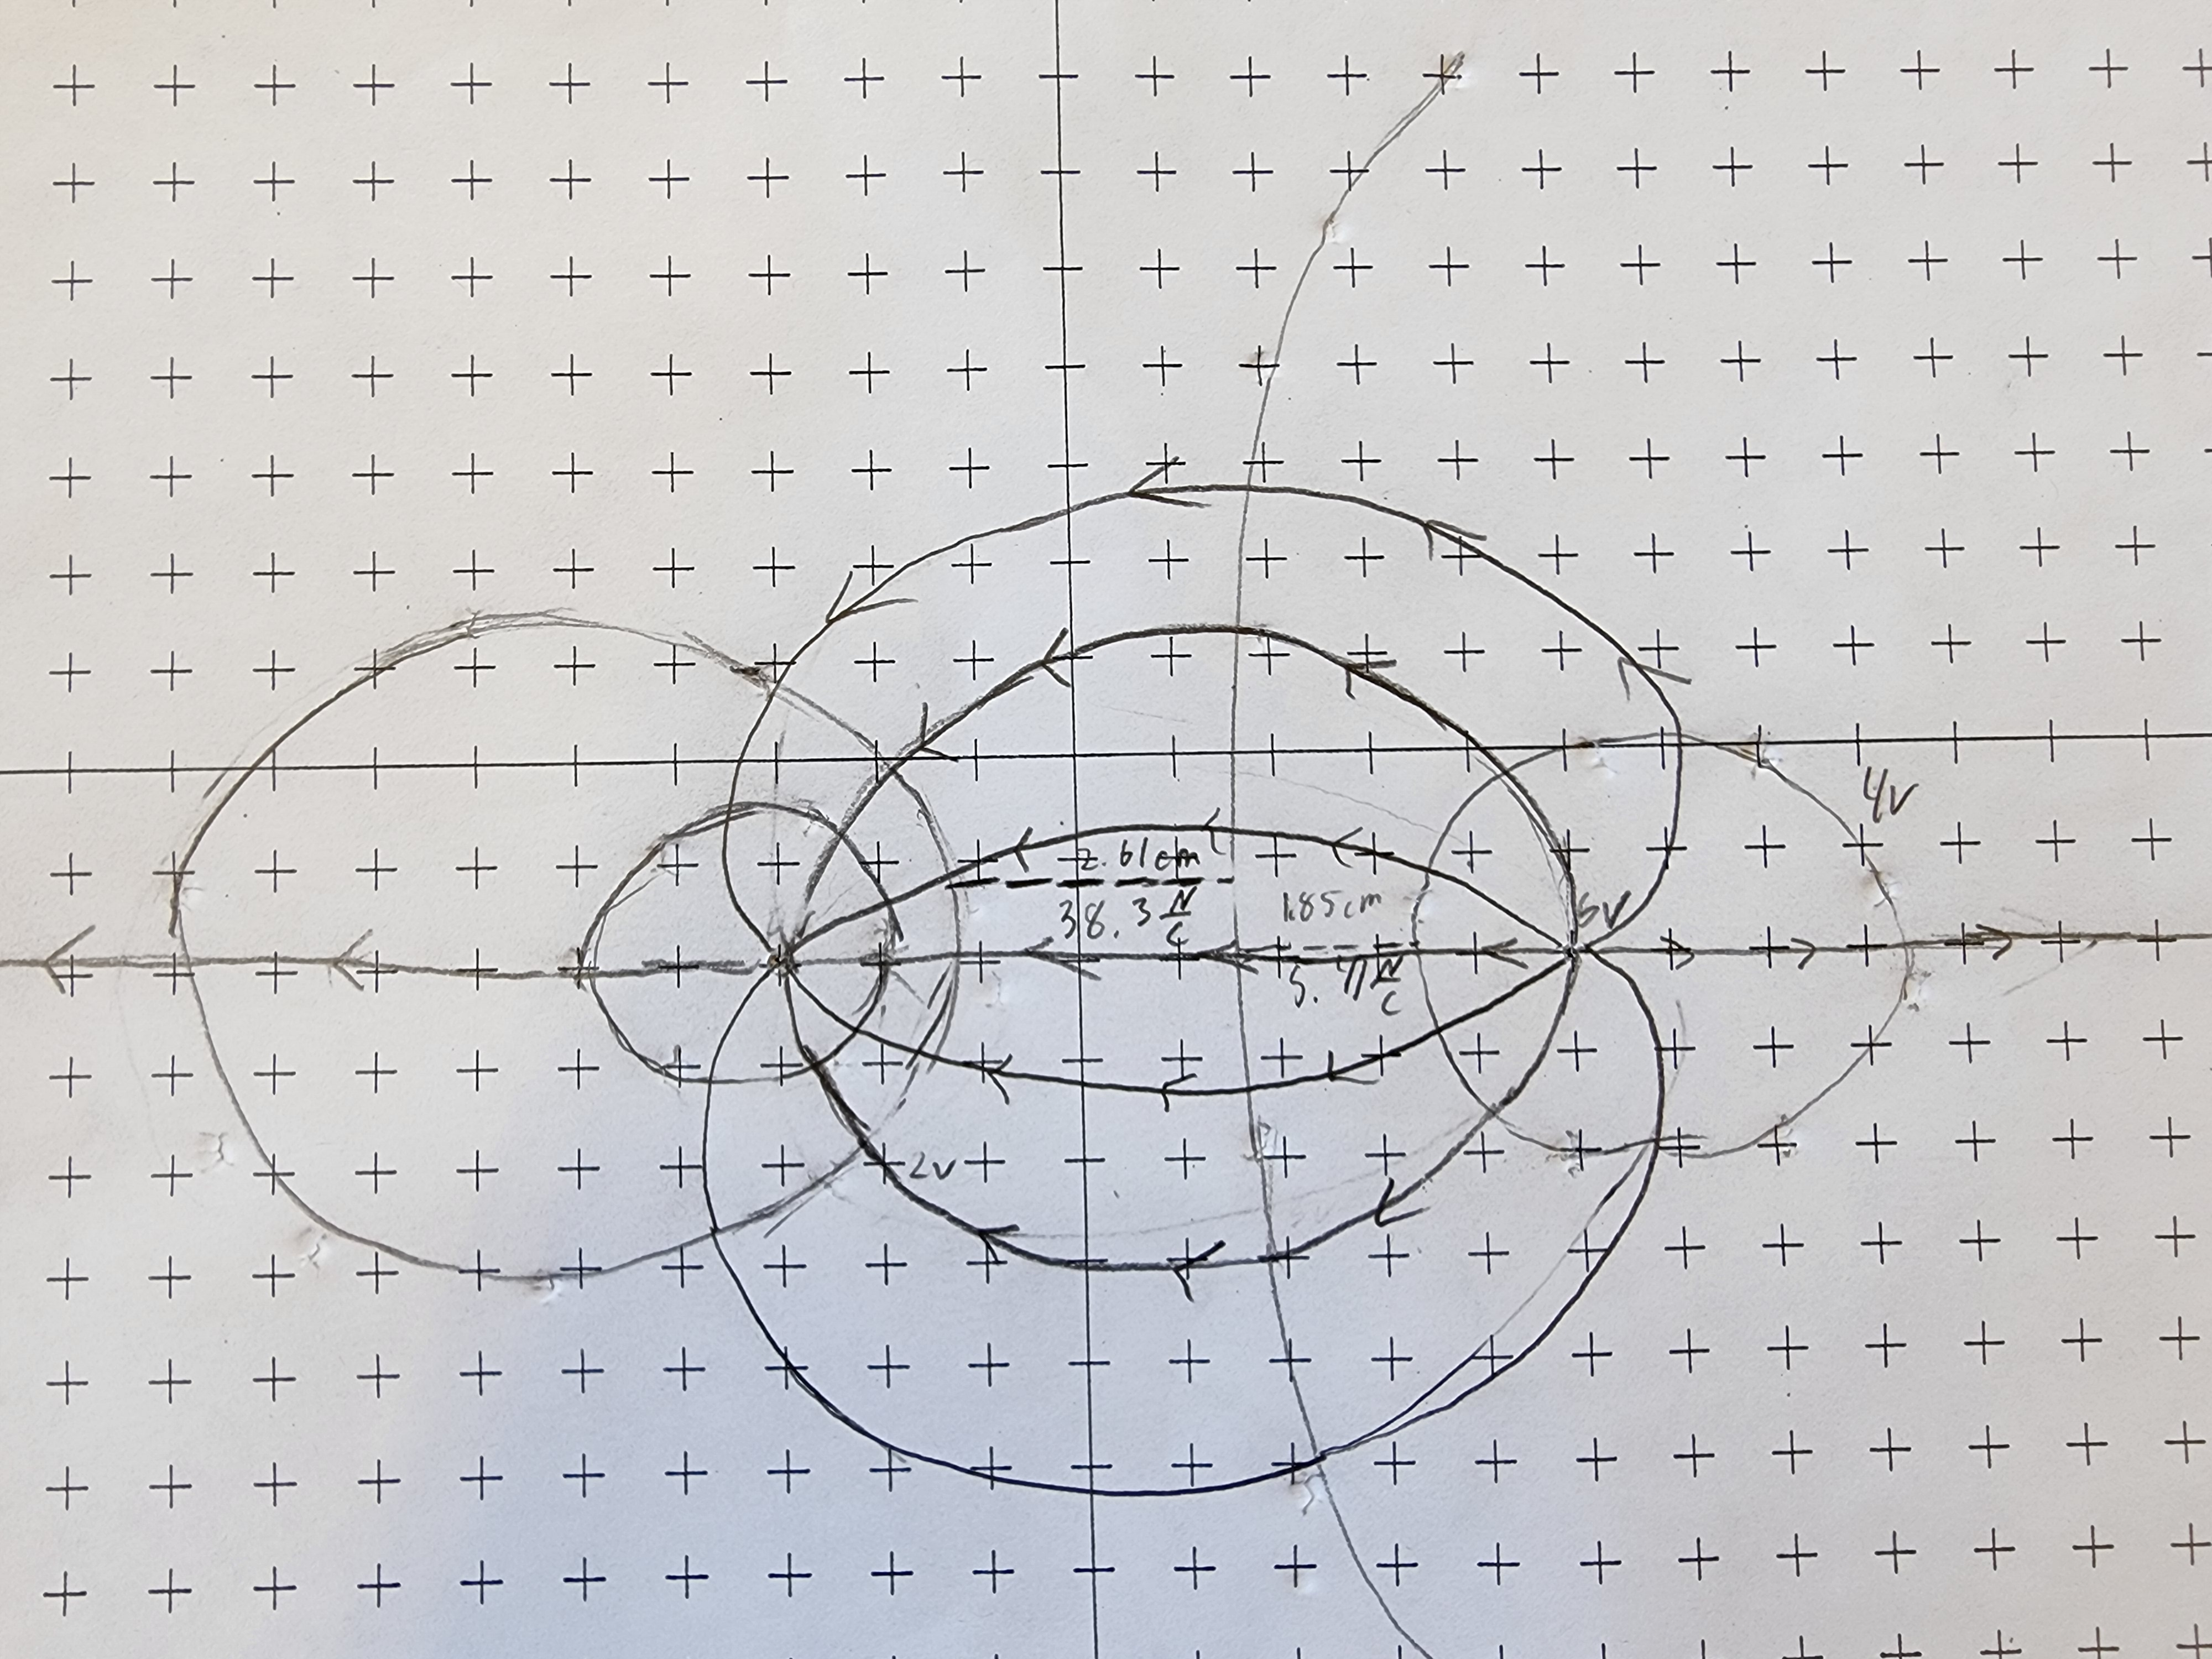
\includegraphics[width=0.8\linewidth]{Ryan's Lines.jpg}
            \caption{Charge distribution, electric field lines, and equipotentials.}
        \end{figure}
        \begin{figure}[H]
            \centering
            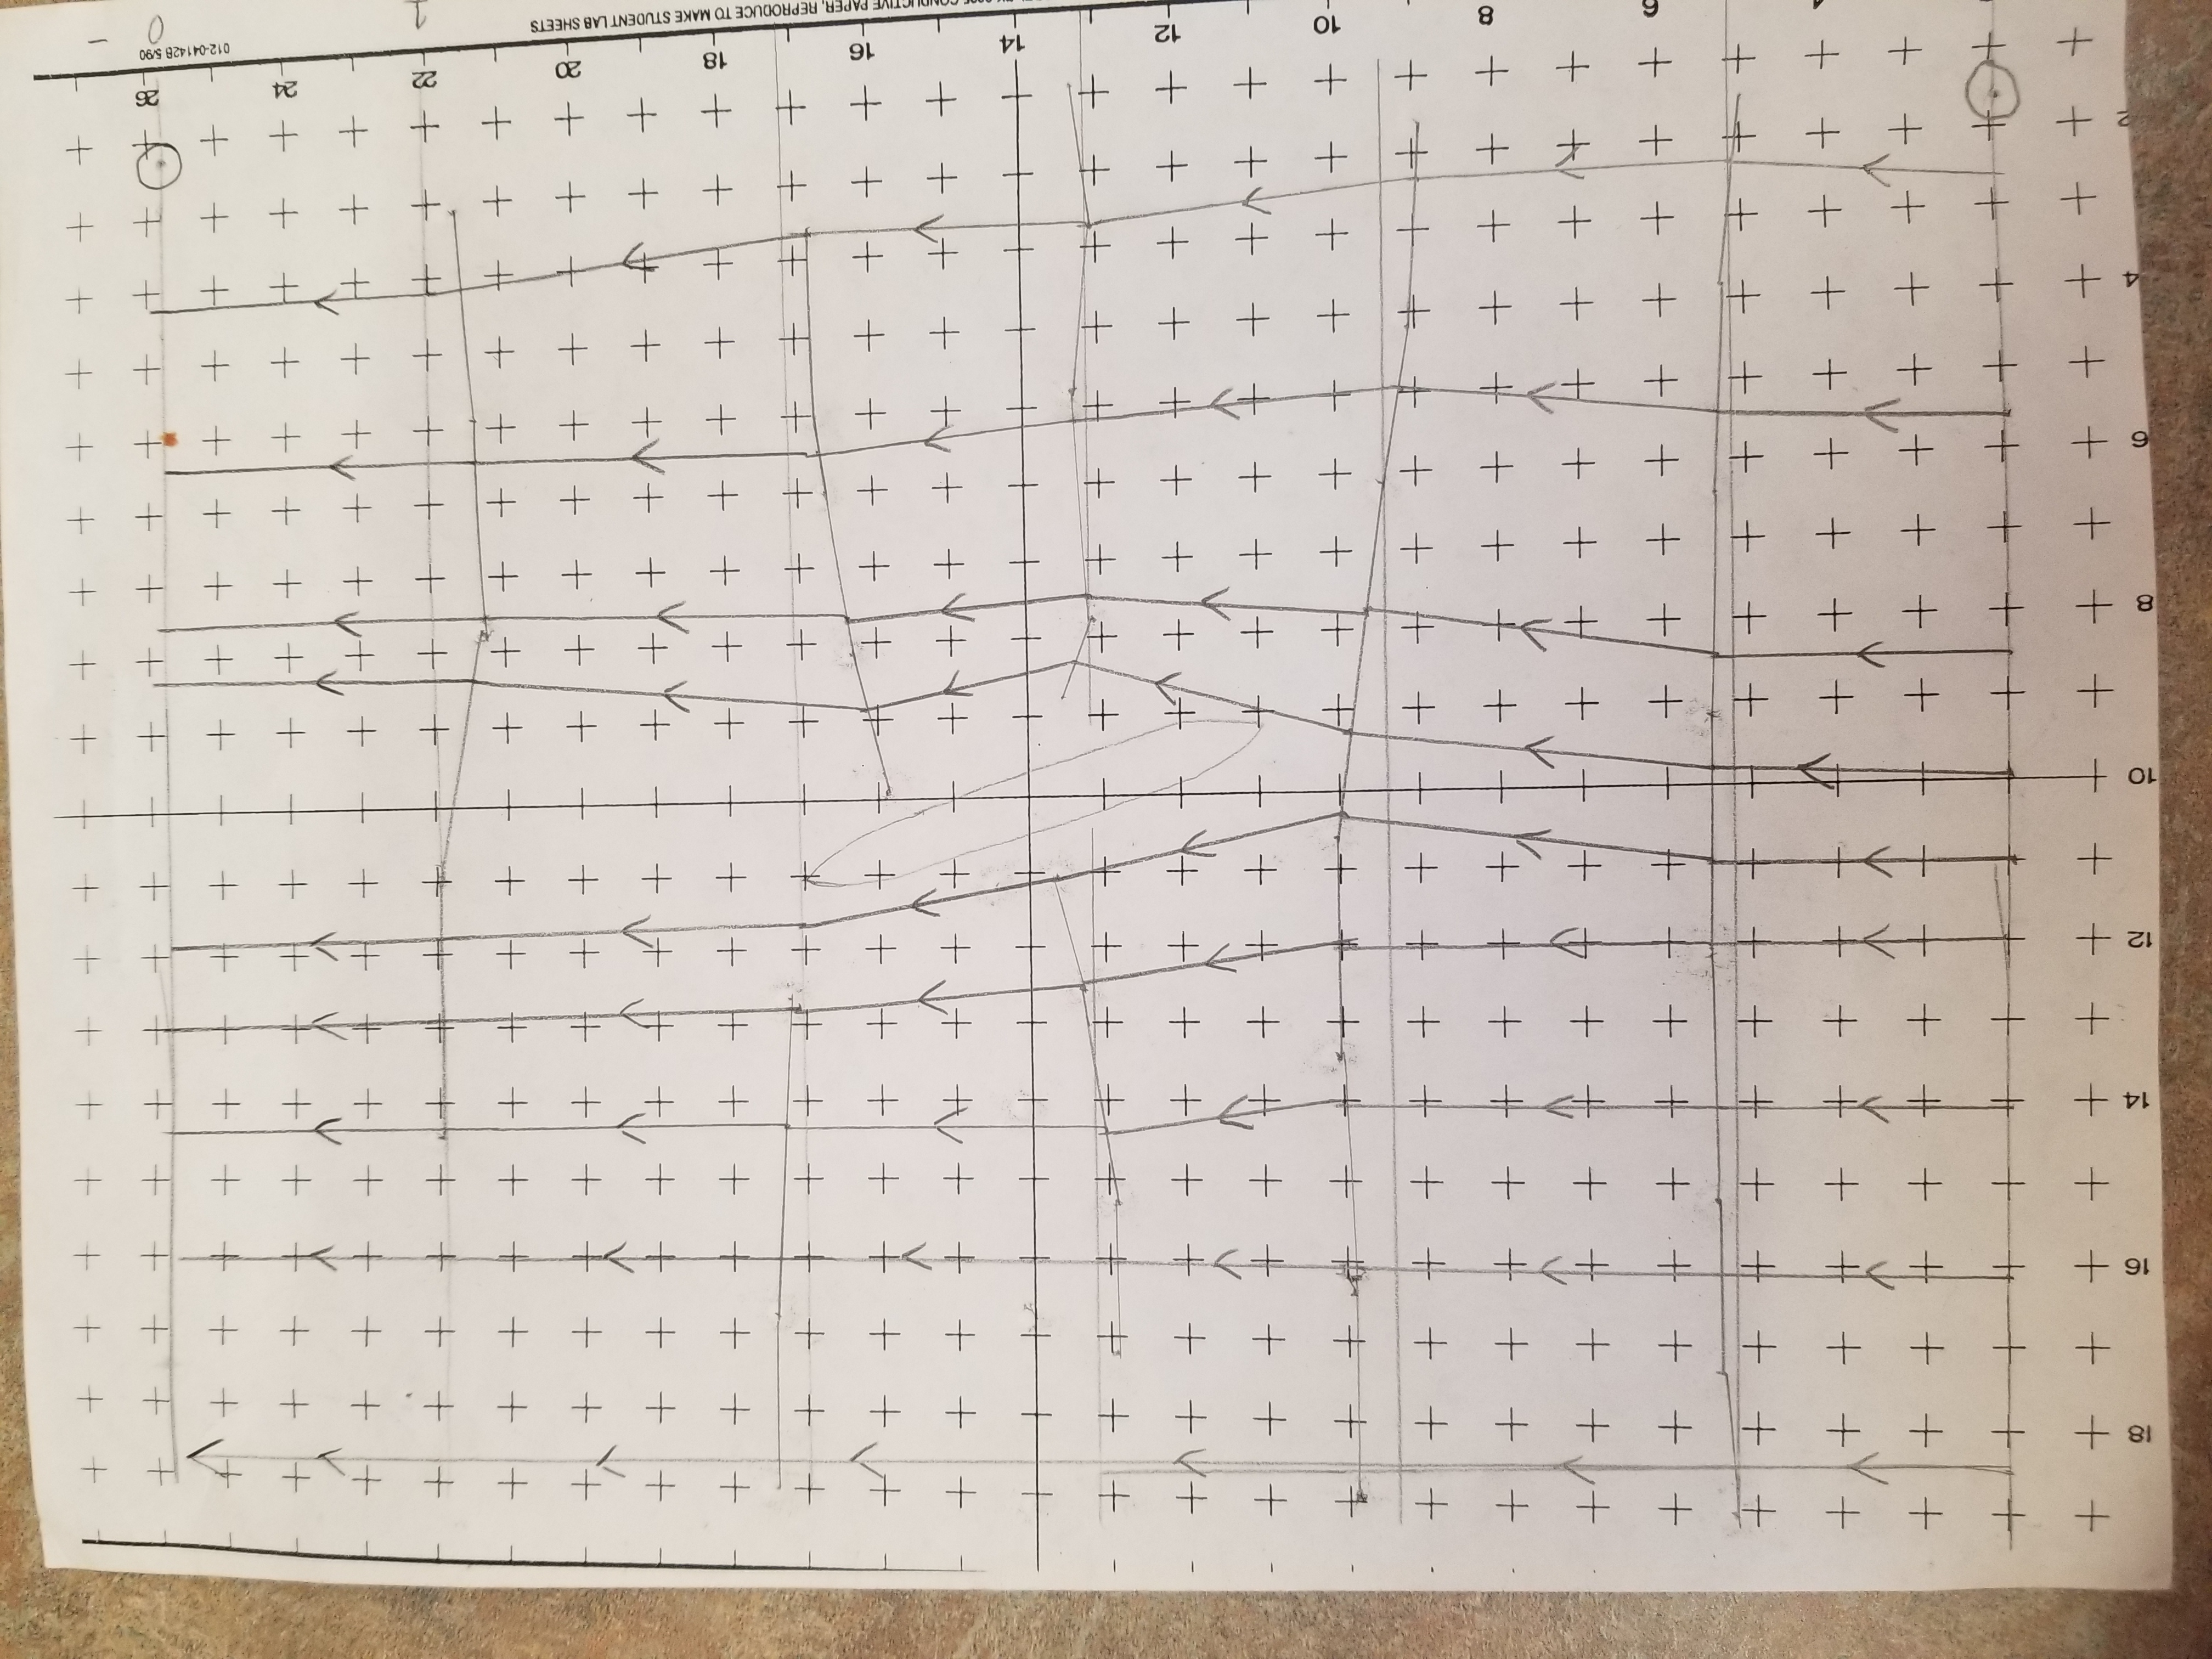
\includegraphics[width=0.8\linewidth]{Ben's Lines.jpg}
            \caption{Charge distribution, electric field lines, and equipotentials.}
        \end{figure}
        \begin{figure}[H]
            \centering
            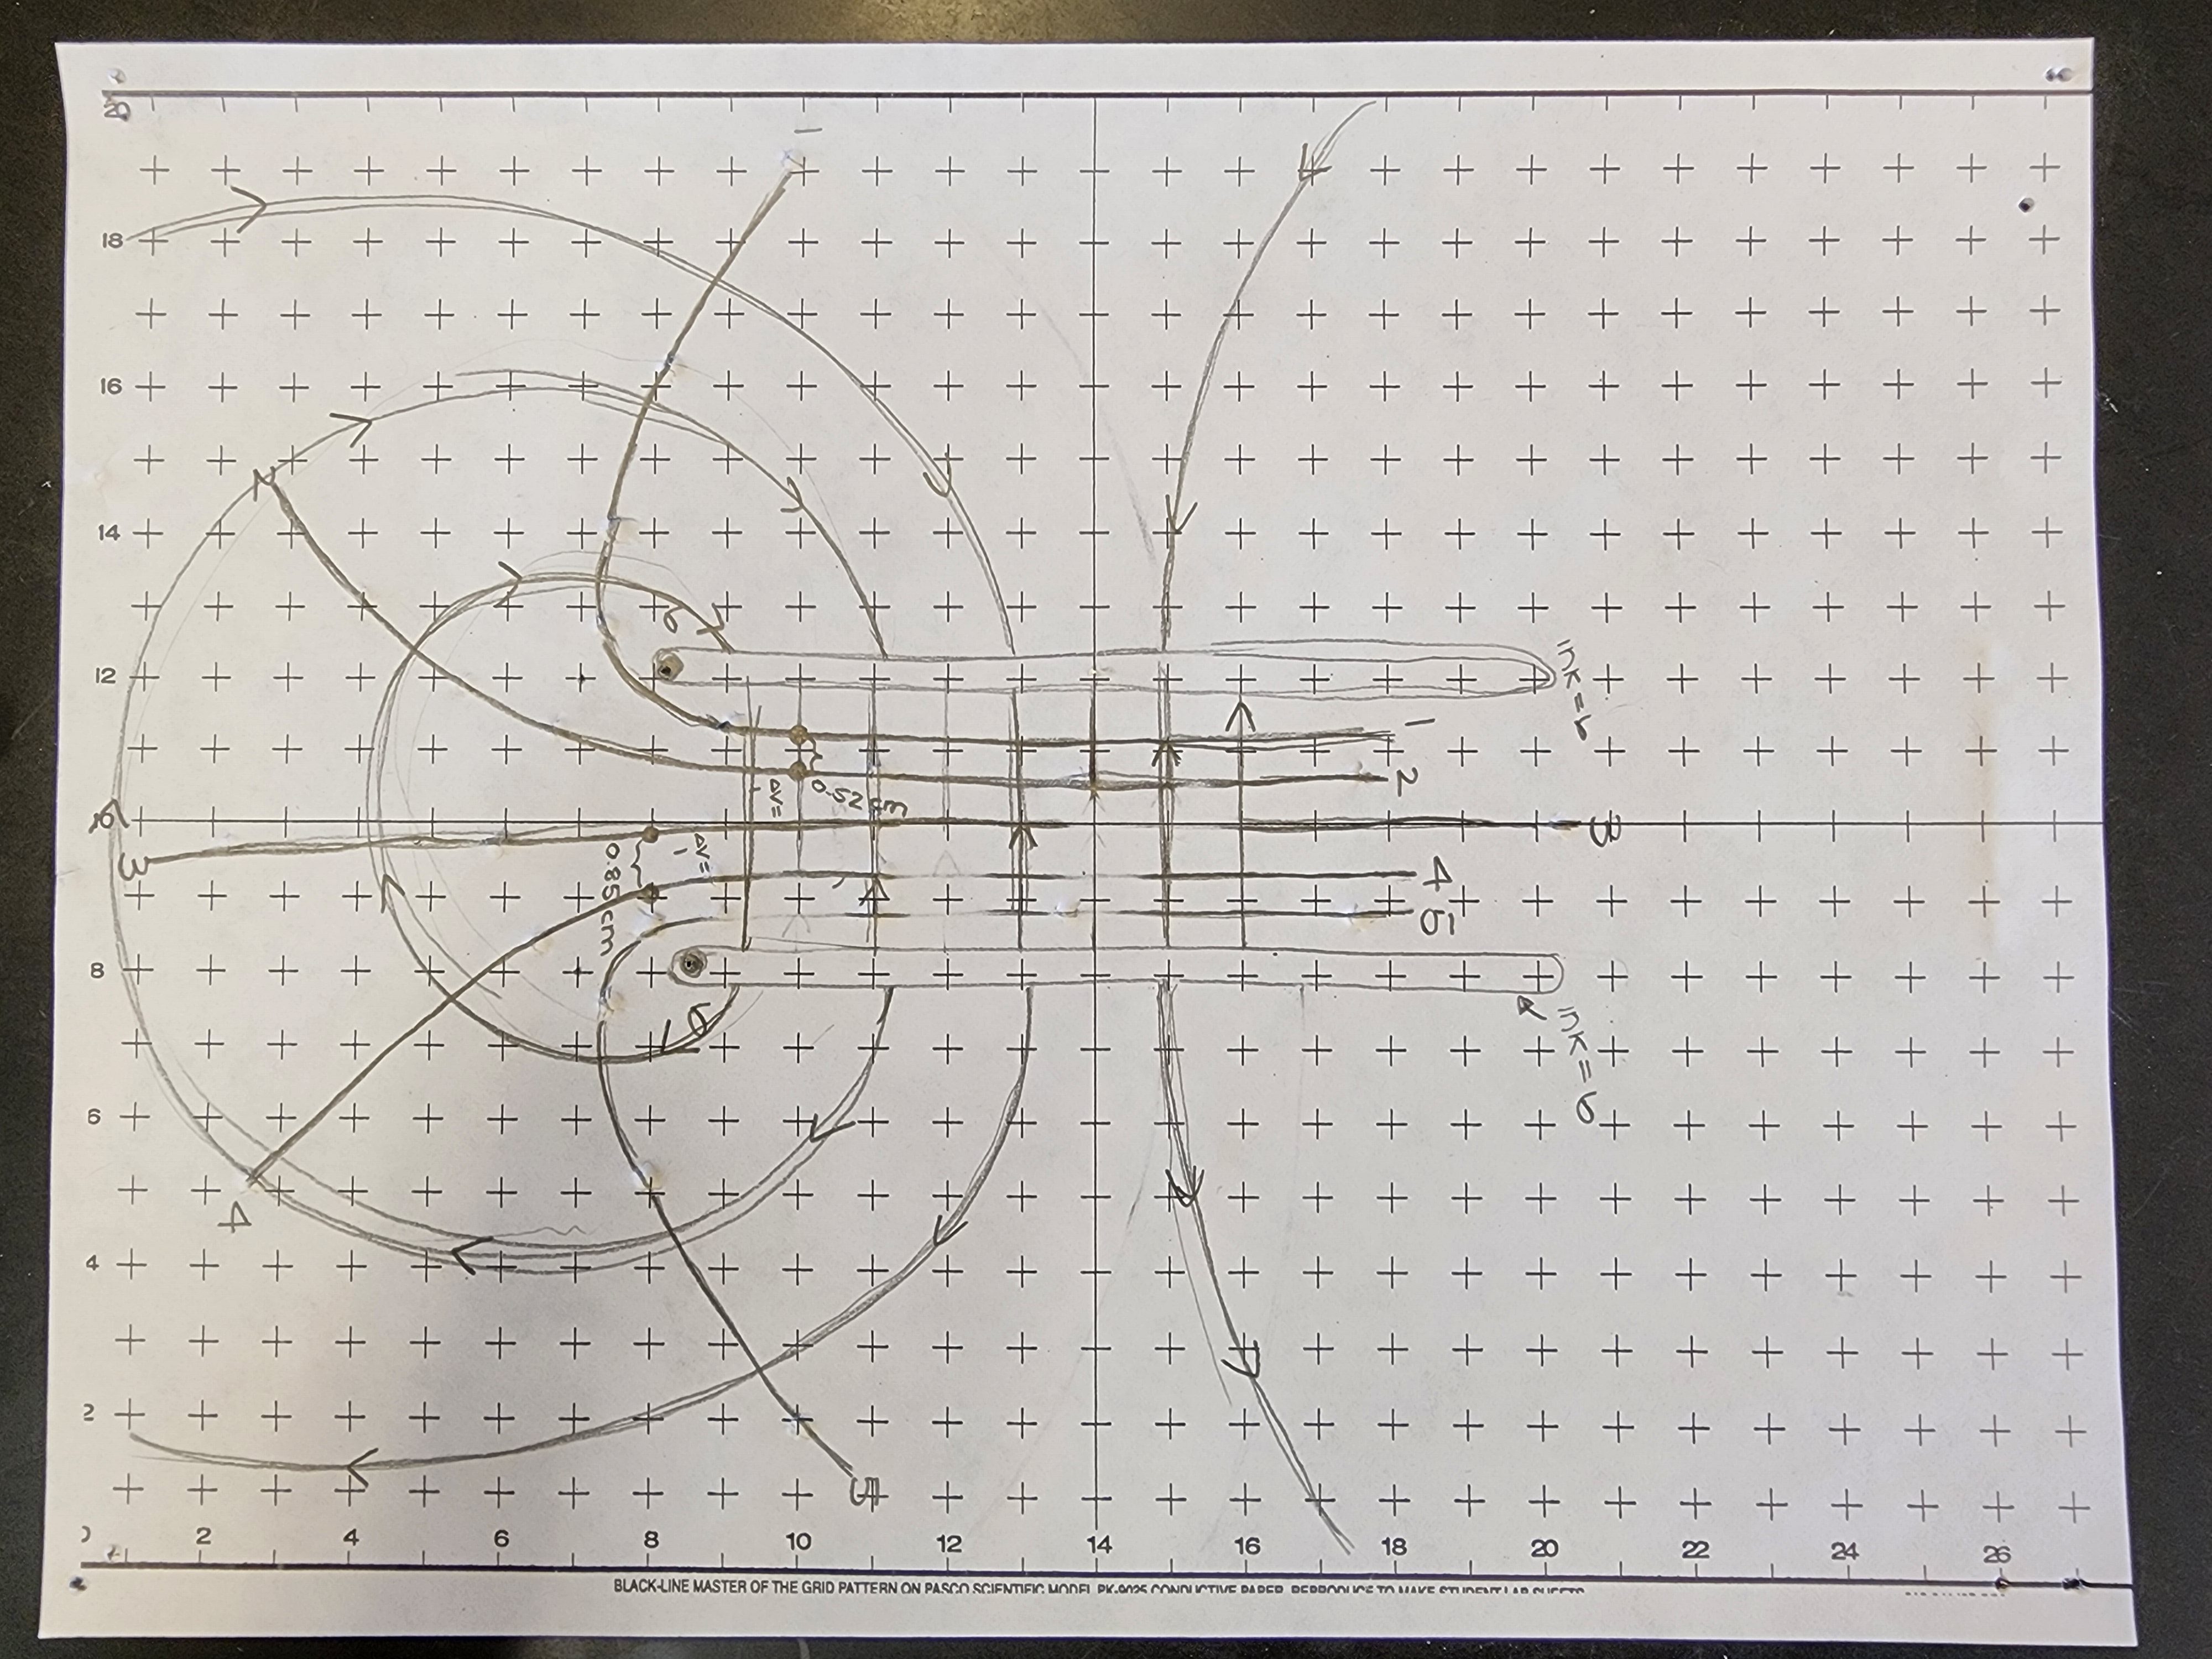
\includegraphics[width=0.8\linewidth]{Erin's Lines.jpg}
            \caption{Charge distribution, electric field lines, and equipotentials.}
        \end{figure}
        \begin{table}[H]
            \centering
            \begin{tabular}{c|c|c|c}
               & \(\Delta s\) (m) & \(\Delta V\) (V) & \(E\) (N/C)\\
               \hline
               1 & 0.0261 & 1 & 38.3\\
               2 & 0.0185 & 1 & 54.1\\
               3 & 0.045 & 1 & 22.3\\
               4 & 0.034 & 1 & 29.4\\
               5 & 0.044 & 1 & 21.7\\
               6 & 0.0052 & 1 & 192\\
               7 & 0.0085 & 1 & 118
            \end{tabular}
        \end{table}
\end{document}